\problemname{Ferry Loading}
A ferry is being loaded with cars, and there's a long line of cars queued up to enter the ferry.
Since the time between the ferry's departures is very long, it's important that as many cars as possible can board the ferry.
The shipping company, Crappy Shippers Inc., has lately recieved a large number of complaints from the organization \emph{Angry Young Algorithmicists}, stating that the packing of the cars on the ferry is \emph{``bad''}, \emph{``suboptimal''}, \emph{``heuristical''} and \emph{``unsustainable''}.
The CEO of the company, Ernst. I. S. Crappy confirms that they have been sloppy about packing the ferry, and has just made a statement that they will always pack the ferry with as many cars as possible.
Ernst said nothing about how they will do this, but there's a rumor floating around that they have requested the assistance of the Swedish Olympiad in Informatics.

The ferry has four lanes, where each lane is a fixed length which is the same for all the lanes.
A line of cars are waiting in a queue to board the ferry, and they will board it in their queuing order.
The staff of the shipping company can decide what lane a car should enter (if it fits).
When a car can't fit in any of the lanes, the ferry is considered full (this means that no car in the queue is ever skipped, even if a later car could fit in some lane).
It's also important that there's a one meter safety margin between cars adjacent in the same lane.

Given the length of the ferry and the lengths of the cars in the queue, help the staff compute the maximum number of cars that can board the ferry.

\begin{figure}[!h]
\begin{center}
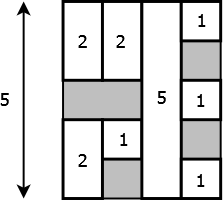
\includegraphics[scale=0.5]{farjan}
\end{center}
\caption{An example of an optimal packing of the ferry. The ferry is $5$ meters long, and the lengths of the cars in the queue are $2, 1, 2, 5, 1, 1, 2, 1, 1, 2$, of which only the first $8$ could fit the ferry.}
\label{fig1}
\end{figure}

\section*{Input}
The first line contains the integer $N$ ($N \le 200$), the number of cars.
The second line contains the integer $L$ ($L \le 60$), the length of the lanes.
This is followed by $N$ integers on a line, where each integer is the length of a car in the same order that they're queuing in.
Each car is between $1$ and $10$ meters long, and does not exceed the length of the ferry.

\section*{Output}
Output a single integer: the maximum number of cars that can board the ferry.

\section*{Scoring}
Your solution will be tested on a set of test case groups.
To get the points for a group, you need to pass all the test cases in the group.

\noindent
\begin{tabular}{| l | l | p{10cm} |}
\hline
Group & Points & Constraints \\ \hline
  $1$    & $40$        & $N \le 20, L \le 40$ \\ \hline 
  $2$    & $60$        & No further constraints. \\ \hline 
\end{tabular}

